\documentclass[11pt]{article}
\usepackage{morefloats}
\usepackage{fullpage}
\usepackage{morefloats}
\usepackage{url}
\usepackage{graphicx}
\usepackage{pdftexcmds}
\usepackage{listings}
\begin{document}

\title{Weekly Updates for Fung Institute Patent Database}
\author{Gabe Fierro\\
	Coleman Fung Institute for Engineering Leadership\\
	UC Berkeley\\
	\texttt{fierro@eecs.berkeley.edu}}
\date{\today}
\maketitle

\section{Introduction}

Here, we discuss the infrastructure and configuration for a weekly process that
downloads the latest weekly releases of USPTO patent files, runs the requisite
data transformations, and integrates the processed data into the larger
database.

This system has not yet been fully adjusted to deal with the weekly application
releases as well as the grant releases, but development is underway and this
document will be updated once those changes are made.

\section{Architecture}

\begin{figure}[h]
\center
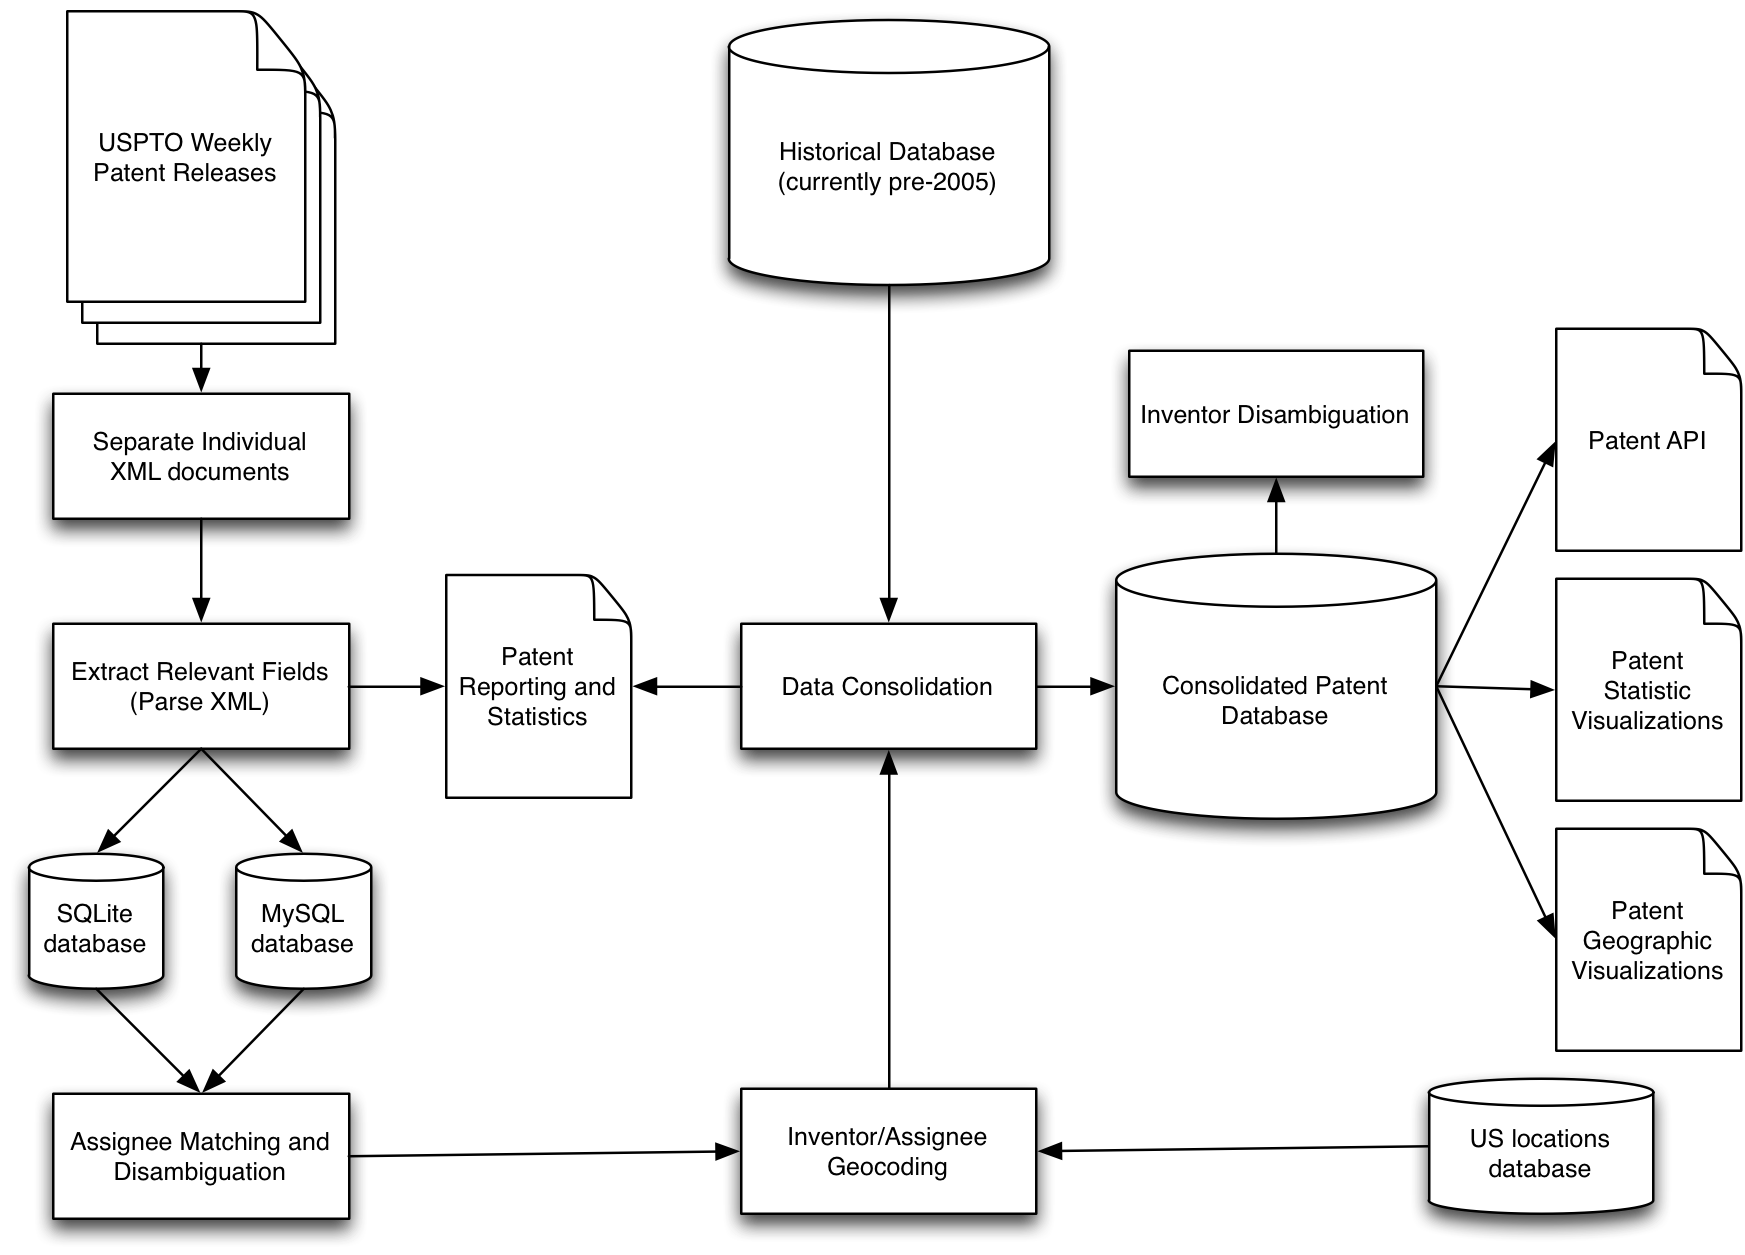
\includegraphics[width=.8\textwidth]{figs/dataprocess}
\caption{Toolchain for processing patents}
\label{fig:dataprocess}
\end{figure}

There are five main stages to the patent processing infrastructure:

\begin{itemize}
    \item \textbf{Parse}: Downloads the latest patent files, interprets the structured data, and inserts the compiled records into the database
    \item \textbf{Clean}: Runs the assignee, lawyer and geographic disambiguations on the data
    \item \textbf{Consolidation}: Prepares the raw inventor data for being sent to the disambiguation engine
    \item \textbf{Disambiguation}: Performs entity resolution on the raw inventor data
    \item \textbf{Integration}: Incorporates the disambiguated inventor records into the database
\end{itemize}

The code represents these stages as modular chunks that can be configured and
run independently of each other. For the weekly update system, these stages
need to be run end-to-end with no interspersed configuration.

At the time of writing, the complete process is not fully automated. The
consolidation stage will output a file \verb`disambiguator.csv` that is
formatted for input into the disambiguation engine. After the disambiguation
engine is run, the integration stage must be run manually. This manual step
will be eliminated once the disambiguator has been properly configured.

% go over the parts of the infrastructure that we're automating
% low memory vs high memory

\section{Configuration}

The `start.py` script provides a simple interface to the patent processor by means of a
configuration file. Here is a sample configuration file:

\begin{verbatim}
[process]
parse=test
clean=True
consolidate=True
outputdir=.
lowmemory=False

[test]
datadir=test/fixtures/xml
dataregex=\d{4}_\d.xml

[2012]
downloaddir=tmpdownload
years=2012
\end{verbatim}

The \verb`[process]` section is mandatory, as it defines the roadmap of the
data process. Each of the lines below the \verb`[process]` line are
configuration options. \verb`parse` indicates which of the parsing
configurations will be run (see below). \verb`clean`, if \verb`True`, runs the
cleaning step on the output of the previously run parse. Similarly,
\verb`consolidate`, if \verb`True`, runs the consolidation step on the output
of the cleaning step. The \verb`lowmemory` option, if \verb`True`, will run the
cleaning and consolidation steps in such a way that they require less memory,
but are slower and sometimes less accurate. It is recommended to leave this as
\verb`True` unless the host computer has more than 64 GB of RAM.

The \verb`parse` section takes as input the title of another configuration
section, which defines the options for which patent files are to be downloaded
and parsed. \verb`parse` sections accept the following configuration options:

\begin{itemize}

    \item \textbf{datadir}: specifies the path to the directory containing the
        XML files that we wish to parse. The path will be evaluated relative to
        the root directory of the preprocessor

    \item \textbf{dataregex}: specifies the regular expression that matches the
        filenames of the XML files we want to parse. This defaults to
        \verb`ipg\d{6}.xml`, which matches USPTO grant files since 2005.

    \item \textbf{years}: specifies the range of years we want to download and
        parse.  If the current year is specified, the script will download all
        possible files. If this option is provided, the \verb`datadir` option
        will be ignored, and the files will be downloaded to the directory
        indicated by the \verb`downloaddir` option (see below). If this option
        is \emph{not} provided, then the parser will operate on the contents of
        \verb`datadir`.

        Years are to be separated by commas, and ranges are indicated by using
        dashes. For example, to download the years 1995, 1997, 1998, 1999,
        2000, 2001 and 2005, we would indicated this as
        \verb`years=1995,1997-2001,2005`.
    
    \item \textbf{downloaddir}: specifies the target directory into which the
        needed patent files will be downloaded. This directory is evaluated
        relative to the root directory of the processor. If it does not exist,
        it will be created. If the directory already exists and already
        contains pre-downloaded files, the process will only download the
        needed files to avoid unnecessary work.

\end{itemize}

The final configuration section, \verb`[xml-handlers]`, specifies which XML
parser is to be used for which files. The USPTO has used eight different data
schemas for patent grants and because it is difficult to automatically detect
the schema of an XML document, this section makes it possible to indicate which
XML parser should be used for which dates of patent releases.

This section should only have to be touched when a new parser is introduced.  A
date is indicated by either YYYY or YYYYMMDD, and ranges are indicated by
dashes in between two dates. If only one date is provided, then the
corresponding parser will be used for all subsequent dates. The current
configuration is listed here:

\begin{verbatim}
[xml-handlers]
2005-20130108=lib.handlers.grant_handler_v42
20130115=lib.handlers.grant_handler_v44
default=lib.handlers.grant_handler_v42
\end{verbatim}

\section{Running}

The installation process has been developed and tested on machines capable of running BASH, which
is Mac OS X and most Linux environments.

To setup a local environment to run the preprocessor, it is best practice to
setup \verb`virtualenv` to handle local Python packages.

\begin{verbatim}
git clone https://github.com/funginstitute/patentprocessor/
cd patentprocessor
pip install virtualenv
virtualenv venv
. venv/bin/activate
pip install -r requirements.txt
\end{verbatim}

Configure the database connection in \verb`lib/alchemy/config.ini`, then
configure the data process in \verb`process.cfg`. The patent processor can then
be started by running \verb`python start.py process.cfg`.

\end{document}
